% !TEX root = ../foresight.tex

\section{Relative pose localization}

\begin{figure}
  \centering
    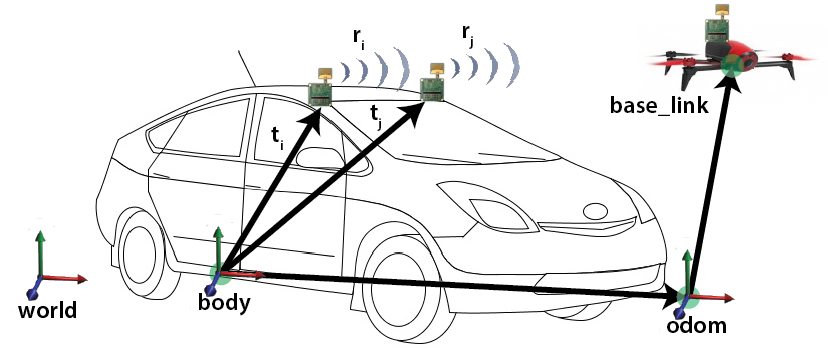
\includegraphics[width=\textwidth]{foresight_frames}
  \caption{The frames and measurements of our system. The base frame
   is the car's body frame. We measure transforms $\bm{t_{i}}$ from the body
   frame to every UWB tag. The velocity controller uses the odom-to-base\textunderscore 
   link transform to calculate commands to control the quadcopter's velocity.
   Planning is done in the car's body frame.
   The UWBs make range measurements $r_{i}$. A position estimate $\bm{\hat{p}}$
   is calculated by solving for the least squares error between $r_{i}$ and $\bm{\hat{p}}$.}
  \label{fig:frames}
\end{figure}

Our planner is concerned with the position $\bm{p}$ and yaw orientation $\psi$
of the quadrotor measured in the car's body frame. We therefore describe the state of the quadrotor as

$$
    x = [\bm{p}, \psi] \in \R^4
$$

We receive a range measurement $r_i$ from each UWB in its own frame. 
From the quadrotor we receive velocity measurements $\bm{v}$ in the odom frame,
a yaw reading $\psi_q$ in the world frame, and an altitude measurement $z_a$ in 
the world frame. Given $n$ UWBs, we define the measurement vector as

$$
   z = [r_1, \dots, r_n, \bm{v}, z_a, \psi_q] \in \R^{n+5}
$$

%We use 6 ultra-wideband radios and the Bebop's onboard odometry measurements
%to estimate the relative position of the quadcopter with respect to the car with an
%accuracy of 13 cm. The 6 UWBs were positioned as far apart as possible on the
%car while still maintaining line of sight with the quadcopter when the
%quadcopter is positioned in front of the car. The transform from a set base position
%on the car to each UWB was then measured. These transforms allow us to
%calculate the distance between each UWB and the estimated state of the quadcopter.


Yaw orientation is calibrated at the start by lining up the quadrotor along the car's x-axis
and measuring the yaw offset $\psi_{off}$ between the car and the quadrotor.
We can therefore calculate $\psi$ as
$$
   \psi = \psi_q - \psi_{off}
$$

One challenge we encountered in estimating the 3D position of the quadrotor was that
the UWBs gave bad readings when the UWB on the quadrotor was out of their plane.
We therefore first estimate $\bm{\hat{p}^{odom}}$ using only use the quadrotor's onboard 
odometry readings $\bm{v}$ and $z_a$ as the inputs to a UKF. We then use the estimated
height, $\bm{\hat{p}_z^{odom}}$ with the UWB range
measurements $r_i$ to estimate the quadrotor's x-y position, $\bm{\hat{p}^{xy}}$.
We do this by first projecting each $r_i$ onto the plane of the estimated height of the quadrotor:

$$
   r_i^{proj} = \sqrt{r_i^2 - (\bm{\hat{p}_z^{odom}})^2}
$$

We then find $\bm{\hat{p}^{xy}}$ by solving the nonlinear least squares optimization

\begin{align*} 
    \min_{{\bm{\hat{p}^{xy}}}} \sum_{i=1}^{n} ((r_{i}^{proj})^2 - \lVert \bm{\hat{p}^{xy}} - \bm{t_i^{xy}}\rVert^2)^2
\end{align*}

with the Jacobian

$$
    J = 4((r_i^{proj})^2 - \lVert \bm{\hat{p}^{xy}} - \bm{t_i^{xy}} \rVert^2)(\bm{t_i^{xy}} - \bm{\hat{p}^{xy}})
$$

We then define the 3D position estimate to be

$$
   \bm{\hat{p}^{ls}} = [\bm{\hat{p}^{xy}}, \hat{z}]
$$

Next, we combine $\bm{\hat{p}^{ls}}$ and $\bm{\hat{p}^{odom}}$ in a second UKF to find
a final position estimate $\bm{\hat{p}}$. Thus the final state estimate is

$$
   \hat{x} = [\bm{\hat{p}}, \psi]
$$











